\documentclass[tikz,border=10pt]{standalone}
\usepackage{amsmath}
\usetikzlibrary{arrows.meta,calc}

\begin{document}
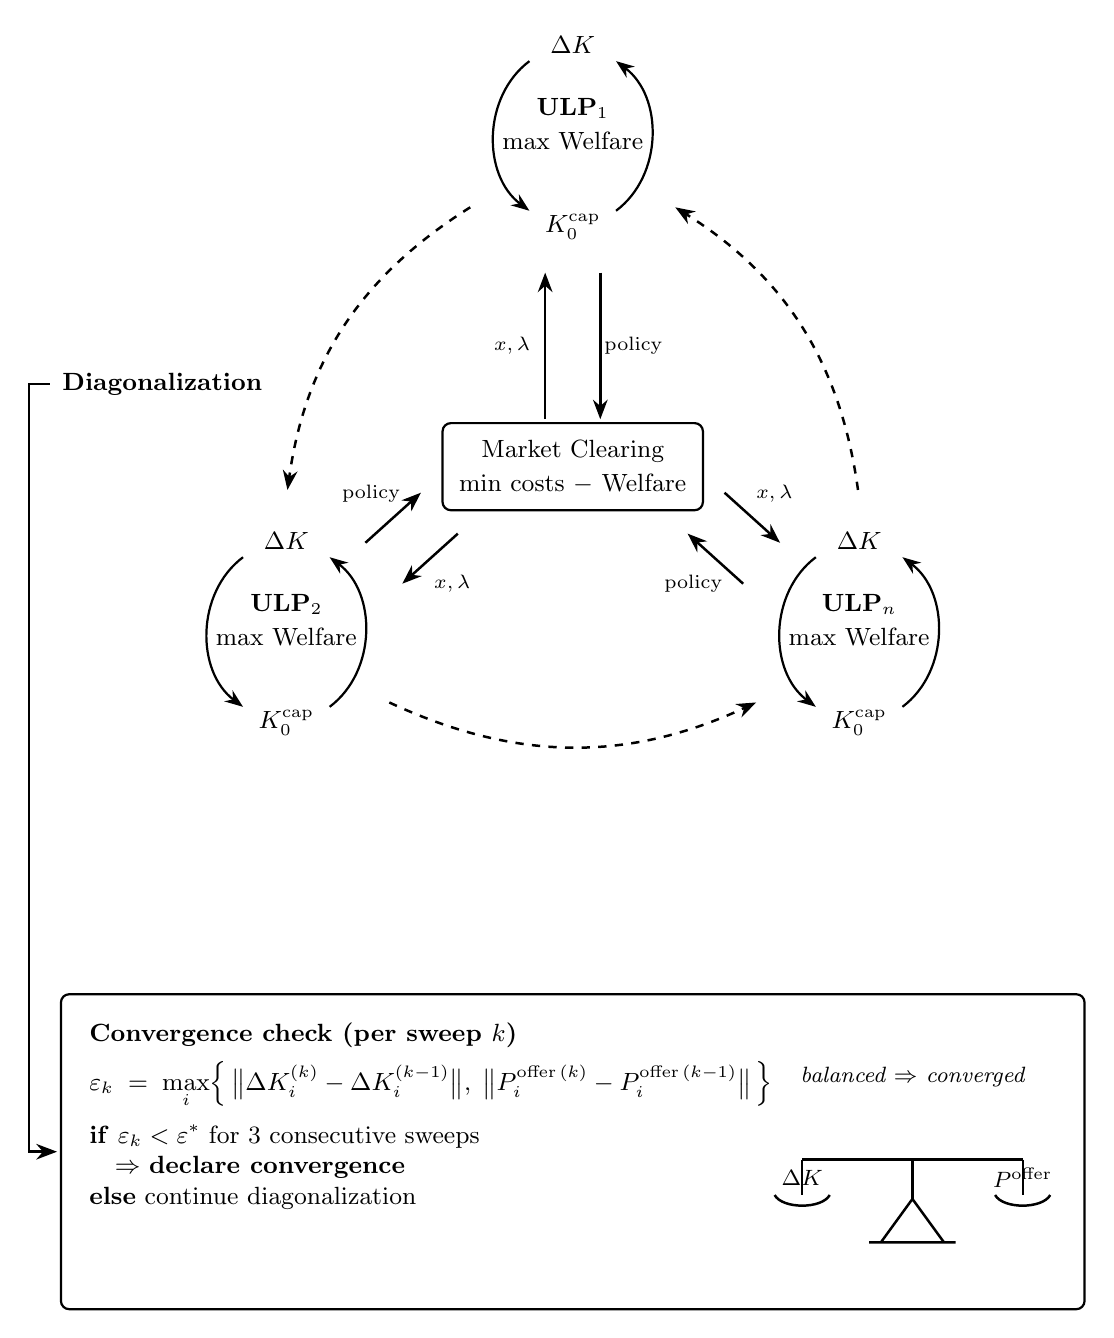
\begin{tikzpicture}[>=Stealth,
    lbl/.style={black, font=\small},
    ttl/.style={black, font=\bfseries\large},
    arr/.style={->, black, line width=0.9pt, shorten >=1pt, shorten <=1pt},
    loop/.style={->, black, line width=0.8pt},
    diag/.style={->, black, line width=0.9pt, dashed,
                 shorten >=3pt, shorten <=3pt},
    diaglbl/.style={black, font=\bfseries\small},
]

% ═══════════════════════════════════════════════════════════════════════
%  Layout
% ═══════════════════════════════════════════════════════════════════════
\def\R{4.2}              % distance from MC to each ULP centre
\def\rx{1.4}             % ULP ellipse x-radius
\def\ry{1.7}             % ULP ellipse y-radius
\def\off{0.35}           % perpendicular offset for parallel arrows

\coordinate (ulp1c) at (90:\R);
\coordinate (ulp2c) at (210:\R);
\coordinate (ulp3c) at (330:\R);
\coordinate (mc)    at (0,0);

% ═══════════════════════════════════════════════════════════════════════
%  ULP macro
% ═══════════════════════════════════════════════════════════════════════
\newcommand{\drawULP}[2]{%
    \node[lbl] at ($(#1)+(0,1.15)$) {$\Delta K$};
    \node[lbl, align=center] at ($(#1)+(0,0.15)$)
        {\textbf{ULP}$_{#2}$\\[0.15em] max Welfare};
    \node[lbl] at ($(#1)+(0,-1.15)$) {$K_0^{\mathrm{cap}}$};
    % K_cap → ΔK on the right
    \draw[loop] ($(#1)+(0.55,-0.95)$)
        .. controls ($(#1)+(1.15,-0.5)$) and ($(#1)+(1.15,0.5)$) ..
        ($(#1)+(0.55,0.95)$);
    % ΔK → K_cap on the left
    \draw[loop] ($(#1)+(-0.55,0.95)$)
        .. controls ($(#1)+(-1.15,0.5)$) and ($(#1)+(-1.15,-0.5)$) ..
        ($(#1)+(-0.55,-0.95)$);
}

\drawULP{ulp1c}{1}
\drawULP{ulp2c}{2}
\drawULP{ulp3c}{n}

% ═══════════════════════════════════════════════════════════════════════
%  Market Clearing box
% ═══════════════════════════════════════════════════════════════════════
\node[lbl, align=center, draw=black, thick, rounded corners=3pt,
      inner sep=6pt] (mcbox) at (mc) {
    Market Clearing\\[0.15em]
    min costs $-$ Welfare
};

% ═══════════════════════════════════════════════════════════════════════
%  ULP ↔ MC arrows  — parallel pairs
%  For each ULP, we compute:
%    - a point on the ULP ellipse facing MC
%    - a point on the MC box facing that ULP
%  Then we offset each endpoint perpendicular to the connecting line
%  so the two arrows (policy out, x,λ in) run parallel.
% ═══════════════════════════════════════════════════════════════════════
\foreach \centre/\ang/\mcanchor in
    {ulp1c/90/north,
     ulp2c/210/south west,
     ulp3c/330/south east}{%
    % endpoints on ULP ellipse (on MC-facing side) and MC box
    \coordinate (ulpEdge) at ($(\centre)+({\ang+180}:{\rx} and {\ry})$);
    \coordinate (mcEdge)  at (mcbox.\mcanchor);

    % Perpendicular offset: take the vector from ulpEdge to mcEdge,
    % rotate by 90°, scale to length \off, then add/subtract from each endpoint.
    % Using the ($ ... $) coordinate calculus with a rotation:
    %   A + (\off * rotate(B-A, 90°))  shifts A perpendicular to AB.
    \coordinate (A1) at ($(ulpEdge)!\off cm!90:(mcEdge)$);
    \coordinate (B1) at ($(mcEdge)!\off cm!-90:(ulpEdge)$);
    \coordinate (A2) at ($(ulpEdge)!\off cm!-90:(mcEdge)$);
    \coordinate (B2) at ($(mcEdge)!\off cm!90:(ulpEdge)$);

    % Midpoints of each arrow
    \coordinate (mid1) at ($(A1)!0.5!(B1)$);
    \coordinate (mid2) at ($(A2)!0.5!(B2)$);

    % Label positions: shift each midpoint perpendicular to its arrow,
    % OUTWARD (away from the other arrow of the pair).
    \def\loff{0.42}  % label offset from arrow line (in cm)
    \coordinate (lbl1) at ($(mid1)!\loff cm!90:(B1)$);
    \coordinate (lbl2) at ($(mid2)!\loff cm!90:(A2)$);

    % policy:  ULP  →  MC
    \draw[arr] (A1) -- (B1);
    \node[lbl, font=\scriptsize] at (lbl1) {policy};

    % x,λ:  MC  →  ULP
    \draw[arr] (B2) -- (A2);
    \node[lbl, font=\scriptsize] at (lbl2) {$x,\lambda$};
}

% ═══════════════════════════════════════════════════════════════════════
%  Diagonalization: dashed cyclic arrows between the ULPs
%  ULP1 → ULP2 → ULPn → ULP1
% ═══════════════════════════════════════════════════════════════════════
% ULP1 → ULP2  (upper-left to lower-left: outer side of both)
\draw[diag]
    ($(ulp1c)+(210:{\rx} and {\ry})$)
    to[bend right=25]
    ($(ulp2c)+(90:{\rx} and {\ry})$);

% ULP2 → ULPn  (bottom arc)
\draw[diag]
    ($(ulp2c)+(330:{\rx} and {\ry})$)
    to[bend right=25]
    ($(ulp3c)+(210:{\rx} and {\ry})$);

% ULPn → ULP1  (right side, returning to top)
\draw[diag]
    ($(ulp3c)+(90:{\rx} and {\ry})$)
    to[bend right=25]
    ($(ulp1c)+(330:{\rx} and {\ry})$);

% ═══════════════════════════════════════════════════════════════════════
%  Diagonalization label — horizontal, placed NEXT TO the left dashed arc
%  (the ULP1 → ULP2 arc).  We pick a point at the midpoint-height of the
%  left arc and shift it outward (to the left) so it sits beside the line
%  rather than on top of it.
% ═══════════════════════════════════════════════════════════════════════
\node[diaglbl, anchor=east] (diaglabel)
    at ($(ulp1c)!0.5!(ulp2c) + (-2.0, 0)$)
    {Diagonalization};

% ═══════════════════════════════════════════════════════════════════════
%  Explanation box below the figure — pseudocode + balance scale
% ═══════════════════════════════════════════════════════════════════════
\coordinate (figBottom) at (0, -\R-\ry-0.3);

% Outer container node: left = pseudocode, right = balance scale
\node[draw=black, thick, rounded corners=3pt, inner sep=0pt,
      minimum width=13cm, minimum height=4cm]
      (explbox) at ($(figBottom) + (0,-2.5)$) {};

% --- LEFT SIDE: pseudocode block ---
\node[anchor=north west, align=left, font=\small]
      at ($(explbox.north west) + (0.25,-0.25)$) {%
    \textbf{Convergence check (per sweep $k$)}\\[0.45em]
    $\displaystyle
      \varepsilon_k \;=\; \max_i \Bigl\{\,
        \bigl\lVert \Delta K_i^{(k)} - \Delta K_i^{(k-1)} \bigr\rVert,\;
        \bigl\lVert P^{\mathrm{offer}\,(k)}_i - P^{\mathrm{offer}\,(k-1)}_i \bigr\rVert
      \,\Bigr\}$\\[0.55em]
    \textbf{if} $\varepsilon_k < \varepsilon^{\ast}$ for $3$ consecutive sweeps\\
    \hspace*{1em}$\Rightarrow$ \textbf{declare convergence}\\
    \textbf{else} continue diagonalization
};

% --- RIGHT SIDE: balance scale ---
% Anchor the scale in the right part of the box.
\coordinate (scaleCtr) at ($(explbox.east) + (-2.2, 0)$);

% pivot (triangle base)
\coordinate (pivot) at ($(scaleCtr) + (0,-0.6)$);
\draw[black, line width=0.9pt]
    ($(pivot)+(-0.55,-0.55)$) -- ($(pivot)+(0.55,-0.55)$)   % ground
    ($(pivot)+(-0.4,-0.55)$)  -- (pivot)                    % left of triangle
    ($(pivot)+(0.4,-0.55)$)   -- (pivot);                   % right of triangle

% balanced beam (perfectly horizontal ⇒ "balanced")
\draw[black, line width=1.1pt]
    ($(pivot)+(-1.4,0.5)$) -- ($(pivot)+(1.4,0.5)$);
% vertical post from pivot up to beam centre
\draw[black, line width=0.9pt]
    (pivot) -- ($(pivot)+(0,0.5)$);

% two pans
\foreach \sgn/\lbltxt in {-1/{$\Delta K$}, 1/{$P^{\mathrm{offer}}$}} {
    \coordinate (panTop) at ($(pivot)+({\sgn*1.4},0.5)$);
    \coordinate (panBase) at ($(panTop)+(0,-0.45)$);
    % suspension line
    \draw[black, line width=0.7pt] (panTop) -- (panBase);
    % pan (shallow bowl)
    \draw[black, line width=0.9pt]
        ($(panBase)+(-0.35,0)$) .. controls
        ($(panBase)+(-0.25,-0.18)$) and
        ($(panBase)+(0.25,-0.18)$) ..
        ($(panBase)+(0.35,0)$);
    % label on pan
    \node[font=\footnotesize] at ($(panBase)+(0,0.22)$) {\lbltxt};
}

% "balanced / converged" caption above the scale
\node[font=\footnotesize\itshape, align=center]
    at ($(scaleCtr)+(0,0.95)$) {balanced $\Rightarrow$ converged};

% Arrow from the "Diagonalization" label down along the left side
% (outside the figure) and then right to the explanation box.
\draw[arr, line width=1pt]
    (diaglabel.west) -- ++(-0.3,0) |- (explbox.west);

\end{tikzpicture}
\end{document}